\documentclass[10pt]{article}
\usepackage[utf8]{inputenc}
\usepackage[T1]{fontenc}
\usepackage{amsmath}
\usepackage{amsfonts}
\usepackage{amssymb}
\usepackage[version=4]{mhchem}
\usepackage{stmaryrd}
\usepackage{bbold}
\usepackage{graphicx}
\usepackage[export]{adjustbox}
\graphicspath{ {./images/} }
\usepackage{caption}

\title{If a generalised butterfly is APN then it operates on 6 bits }

\author{Anne Canteaut ${ }^{1}$, Léo Perrin ${ }^{1}$, Shizhu Tian ${ }^{1,2,3}$\\
${ }^{1}$ Inria, Paris, France.\\
${ }^{2}$ State Key Laboratory of Information Security, Institute of Information Engineering, Chinese Academy of Sciences, Beijing, China\\
${ }^{3}$ School of Cyber Security, University of Chinese Academy of Sciences, Beijing, China\\
\{firstname.lastname\}@inria.fr}
\date{}


\begin{document}
\maketitle
\captionsetup{singlelinecheck=false}


\section*{To cite this version:}
Anne Canteaut, Léo Perrin, Shizhu Tian. If a generalised butterfly is APN then it operates on 6 bits. Cryptography and Communications - Discrete Structures, Boolean Functions and Sequences, 2019, 11 (6), pp.1147-1164. $\langle 10.1007 / \mathrm{s} 12095-019-00361-\mathrm{x}\rangle .\langle$ hal-02420992 $\rangle$

\section*{HAL Id: hal-02420992 \\
 https://inria.hal.science/hal-02420992v1}
Submitted on 20 Dec 2019

HAL is a multi-disciplinary open access archive for the deposit and dissemination of scientific research documents, whether they are published or not. The documents may come from teaching and research institutions in France or abroad, or from public or private research centers.

L'archive ouverte pluridisciplinaire HAL, est destinée au dépôt et à la diffusion de documents scientifiques de niveau recherche, publiés ou non, émanant des établissements d'enseignement et de recherche français ou étrangers, des laboratoires publics ou privés.

\section*{If a Generalised Butterfly is APN then it Operates on 6 Bits }


\begin{abstract}
Whether there exist Almost Perfect Non-linear permutations (APN) operating on an even number of bit is the so-called Big APN Problem. It has been solved in the 6-bit case by Dillon et al. in 2009 but, since then, the general case has remained an open problem.\\
In 2016, Perrin et al. discovered the butterfly structure which contains Dillon et al.'s permutation over $\mathbb{F}_{2^{6}}$. Later, Canteaut et al. generalised this structure and proved that no other butterflies with exponent 3 can be APN. Recently, Yongqiang et al. further generalized the structure with Gold exponent and obtained more differentially 4-uniform permutations with the optimal nonlinearity. However, the existence of more APN permutations in their generalization was left as an open problem.\\
In this paper, we adapt the proof technique of Canteaut et al. to handle all Gold exponents and prove that a generalised butterfly with Gold exponents over $\mathbb{F}_{2^{2 n}}$ can never be APN when $n>3$. More precisely, we prove that such a generalised butterfly being APN implies that the branch size is strictly smaller than 5 . Hence, the only APN butterflies operate on 3-bit branches, i.e. on 6 bits in total.
\end{abstract}

Keywords. Boolean function, Sbox, APN, Differential uniformity, Butterflies

\section*{1 Introduction}
S(ubstitution)-boxes are core components in symmetric ciphers where they serve as the confusion part. In most cases, they are their only nonlinear components. In order for the algorithm to resist the two most prominent cryptanalysis techniques, namely differential [2,3] and linear attacks [13], S-boxes should have a low differential uniformity [14] and a high nonlinearity [7].

Let $F$ be a function from $\mathbb{F}_{2}^{m}$ into $\mathbb{F}_{2}^{m}$. We say that $F$ is differentially $\delta$-uniform if, for any nonzero $a$ in $\mathbb{F}_{2}^{m}$ and $b \in \mathbb{F}_{2}^{m}$, the equation $F(x)+F(x+a)=b$ has at most $\delta$ solutions in $\mathbb{F}_{2}^{m}$. The lower bound for functions on $\mathbb{F}_{2}^{m}$ is 2, and the functions that achieve this bound are called Almost Perfect Nonlinear (APN) [15]. That is, a function $F: \mathbb{F}_{2}^{m} \rightarrow \mathbb{F}_{2}^{m}$ is APN if the following equation has at most two solutions:

$$
F(x)+F(x+a)=b
$$

for any $b \in \mathbb{F}_{2}^{m}$ and any $a \in \mathbb{F}_{2}^{m}$ such that $a \neq 0$. An APN permutation over $\mathbb{F}_{2}^{m}$ would be an S-box providing optimal protection against differential attacks. Such components are easy to find for $m$ odd: the Gold functions $x \mapsto x^{2^{i}+1}$ and the inverse mapping $x \mapsto x^{2^{m}-2}$, which are defined by identifying $\mathbb{F}_{2^{m}}$ with $\mathbb{F}_{2}^{m}$, are APN permutations in this case. However, the very existence of APN permutations operating on an even number of bits is an open problem nicknamed the big APN problem.

Open Problem 1 (Big APN Problem). Is there an APN permutation of $\mathbb{F}_{2^{m}}$ where $m=2 n$ ?

It has been an open problem in the field of vectorial Boolean functions since Nyberg introduced the differential uniformity in the early 90 's [14].

Some negative results are known. For instance, Hou proved in [10] that there are no APN permutations over $\mathbb{F}_{2^{4}}$ and that there are no APN permutations over $\mathbb{F}_{2^{2 n}}$ with coefficients in $\mathbb{F}_{2^{n}}$. Also, an APN permutation over $\mathbb{F}_{2^{2 n}}$ cannot neither be a monomial function nor a quadratic function [1].

The only known solution to this problem is a sporadic case found by Dillon et al. [4] for $m=6$. At the time of writing, it remains the only known APN permutation over $\mathbb{F}_{2^{2 n}}$. This solution was constructed by finding a permutation in the CCZ-equivalence class of a known quadratic APN function, namely the Kim mapping $x \mapsto x^{3}+x^{10}+g x^{24}$ where $g$ is a root of the primitive polynomial used to define $\mathbb{F}_{2^{6}}$.

To try and use a similar approach, Yu et al. [17] designed a new matrix-based method to generate quadratic APN functions. They obtained 8157 new quadratic APN functions over $\mathbb{F}_{2^{8}}$. However, none of these APN functions are CCZ-equivalent to permutations.

In [16], Perrin et al. identified a specific structure called Open Butterfly which is affineequivalent to Dillon et al.'s permutation. This structure is easily defined over higher dimensions, but, unfortunately, Canteaut et al. [5] proved that an even broader family of permutations containing the butterflies of Perrin et al. did not contain any APN permutations for $m>6$.

Several teams then studied other generalizations of the original butterfly of [16]. Firstly, it was shown in [8] that changing the exponent from 3 to $2^{i}+1$ in the construction of Perrin et al. still yielded differentially 4 -uniform permutations. Then, Li et al. showed that the generalization of Canteaut et al. had the same properties [11], and that this family of generalised butterflies contains some functions which are not CCZ-equivalent to the functions studied in [5]. In each case, the authors established that such generalizations have a differential uniformity at most equal to 4 except in some sporadic cases but they left the existence of APN permutations among them as an open problem. In this paper, we answer this question by proving the following theorem.

Theorem 1. If a generalised butterfly is $A P N$ then it operates on 6 bits.\\
In other words, natural quadratic generalizations of the initial structure of Perrin et al. do not provide any new solutions to the big APN problem.

The remainder of the paper is our proof of this theorem. First, we formally describe generalized butterflies and some of their basic properties in Section 2. Then, in Section 3, we present some useful propositions, both new ones and from the literature, which will be used further in the paper. Our proof then operates in two high level steps. In Section 4, we establish a necessary criterion for a butterfly to be APN which we call the refined trace condition. Then, in Section 5, we show that this condition implies that the block size is upperbounded by 6 so that Theorem 1 holds.

\section*{2 Generalised Butterflies}
In this section, we formally define the generalisation of the butterfly structure we consider in this paper and establish some of its most basic properties.

\subsection*{2.1 Definition}
In the remainder of the paper, we consider an even integer $m=2 n$ which is not divisible by 4 , i.e., $n$ is always odd. Also, vectorial Boolean functions from $\mathbb{F}_{2}^{m}$ into $\mathbb{F}_{2}^{m}$ are identified with mappings from $\mathbb{F}_{2^{n}} \times \mathbb{F}_{2^{n}}$ to itself. It is worth noticing that the choice of the basis used for identifying $\mathbb{F}_{2^{n}}$ with $\mathbb{F}_{2}^{n}$ does not affect the cryptographic properties of the functions we are studying since different bases lead to functions which are affine-equivalent.

We now define the family of vectorial functions that will be studied in the paper.\\
Definition 1 (Generalised Butterflies). Let $R$ be a bivariate polynomial of $\mathbb{F}_{2^{n}}$ such that $R_{y}$ : $x \mapsto R(x, y)$ is a permutation of $\mathbb{F}_{2^{n}}$ for all $y$ in $\mathbb{F}_{2^{n}}$. The closed butterfly $\bigvee_{R}$ is the function of $\left(\mathbb{F}_{2^{n}}\right)^{2}$ defined by

$$
\bigvee_{R}(x, y)=(R(x, y), R(y, x))
$$

and the open butterfly $\mathrm{H}_{R}$ is the permutation of $\left(\mathbb{F}_{2^{n}}\right)^{2}$ defined by

$$
\mathrm{H}_{R}(x, y)=\left(R_{R_{y}^{-1}(x)}(y), R_{y}^{-1}(x)\right)
$$

where $R_{y}(x)=R(x, y)$ and $R_{y}^{-1}\left(R_{y}(x)\right)=x$ for any $x, y$. A representation of $\mathrm{H}_{R}$ is given in Figure 1a and one of $\bigvee_{R}$ is given in Figure 1b.

\begin{figure}[h]
\begin{center}
  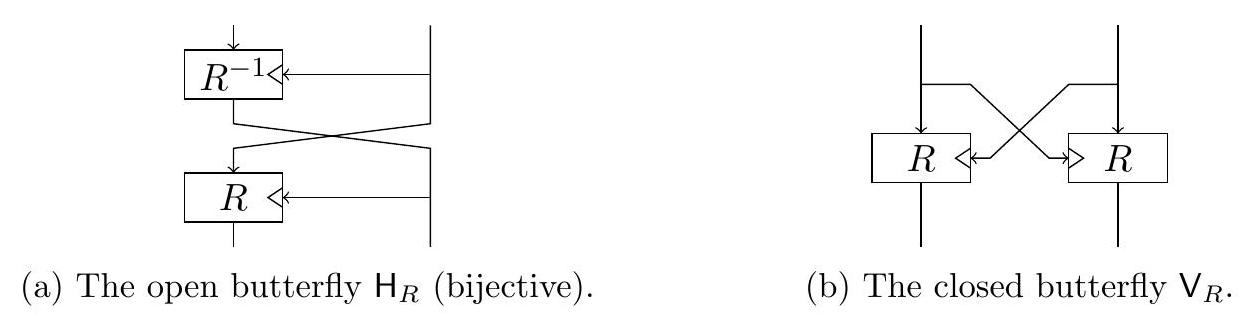
\includegraphics[alt={},max width=\textwidth]{394c8434-d51f-4c8e-a765-d0e2d6dd21e2-04_332_1252_863_370}
\captionsetup{labelformat=empty}
\caption{Figure 1: The butterfly constructions.}
\end{center}
\end{figure}

It can be easily checked that, for any choice of the keyed permutation $R$, the open butterfly $\mathrm{H}_{R}$ is an involution and, as such, a permutation.

Several particular cases of this structure have been presented in the literature. They consist in iterative generalizations of the first butterfly structure which was introduced in [16].

\begin{itemize}
  \item In [16], Perrin et al. found that Dillon et al.'s permutation is affine equivalent to $\mathrm{H}_{R}$ with $R_{y}(x)=(x+\alpha y)^{3}+y^{3}$, for $n=3$, where $\operatorname{Tr}(\alpha)=0$. They showed that such structures always have algebraic degree $n+1$ and a differential uniformity at most equal to 4 whenever $\alpha \neq 0$ and $n$ is odd. However, they left their nonlinearity as an open problem along with the existence of APN permutations for $n>3$ among them.
  \item Canteaut et al. [5] considered the broader class of polynomials $R_{y}(x)=(x+\alpha y)^{3}+\beta y^{3}$ which, up to equivalence, contains all $R$ of degree 3 such that $R_{y}$ is always a permutation. They showed that it was always differentially 4 (except for some sporadic cases) and that it could only be APN when $n=3$. They also showed that the nonlinearity of butterflies was always equal to the best known one (except for some sporadic cases). Their results are trivially generalized to exponents of the form $3 \times 2^{i}$.
  \item Fu et al. [8] instead chose to look at different exponents, i.e. at $R_{y}=(x+\alpha y)^{2^{i}+1}+y^{2^{i}+1}$ with $\operatorname{gcd}(i, n)=1$. They showed that, again, such structures were always differentially 4-uniform and always have the best nonlinearity known to be possible. They also proved that the closed butterfly with $\alpha=1$ was always a permutation.
  \item Li et al. [11] investigated the broadest class of butterflies, namely those with $R_{y}=(x+ \alpha y)^{2^{i}+1}+\beta y^{2^{i}+1}$ with $\operatorname{gcd}(i, n)=1$. They showed that, except in some sporadic cases, the nonlinearity of such constructions was the best known to be possible and the differential uniformity was at most 4 . However, they left the existence of APN functions among them as an open problem.
\end{itemize}

In this paper, we focus on the broadest definition, i.e. on the case where

$$
R_{y}=(x+\alpha y)^{2^{i}+1}+\beta y^{2^{i}+1}
$$

with $\operatorname{gcd}(i, n)=1$. As Li et al. already proved that such structures yield the best known nonlinearity and differential uniformity, we focus only on whether they can be APN or not.

\subsection*{2.2 Equivalence Relations}
To begin with, we recall some basic notations of equivalence relations among vectorial Boolean functions. Two functions $F_{1}, F_{2}$ from $\mathbb{F}_{2}^{m}$ into $\mathbb{F}_{2}^{m}$ are $E$ (xtended) $A$ (ffine)-equivalent if there exist two affine permutations $A_{1}, A_{2}$ from $\mathbb{F}_{2}^{m}$ into $\mathbb{F}_{2}^{m}$ and an affine function $A_{3}$ from $\mathbb{F}_{2}^{m}$ into $\mathbb{F}_{2}^{m}$ such that

$$
F_{1}(x)=A_{1}\left(F_{2}\left(A_{2}(x)\right)\right)+A_{3}(x)
$$

A more general framework is introduced by considering the graphs of the functions [6]. Two functions $F_{1}, F_{2}$ from $\mathbb{F}_{2}^{m}$ into $\mathbb{F}_{2}^{m}$ are called CCZ-equivalent (after Carlet, Charpin and Zinoviev) if there exists an affine permutation $\mathcal{L}$ over $\mathbb{F}_{2}^{2 m}$ such that

$$
\mathcal{L}\left(\left\{\left(x, F_{1}(x)\right), \forall x \in \mathbb{F}_{2}^{m}\right\}\right)=\left\{\left(x, F_{2}(x)\right), \forall x \in \mathbb{F}_{2}^{m}\right\}
$$

Both the differential uniformity and the nonlinearity are invariant under both EA-equivalence and CCZ-equivalence. In particular, all functions CCZ-equivalent to an APN function are APN themselves.

As in the case studied in [5], the generalised butterflies with $R_{y}(x)=(x+\alpha y)^{2^{i}+1}+\beta y^{2^{i}+1}$ are linked by the following relations.

\begin{itemize}
  \item If the exponent is equal to $e=\left(2^{i}+1\right) \times 2^{t}$, the corresponding closed butterfly is affineequivalent to the closed butterfly with $e=2^{i}+1$ and the same $\alpha, \beta$. Therefore, all results presented in the paper also hold when
\end{itemize}

$$
R(x, y)=(x+\alpha y)^{\left(2^{i}+1\right) \times 2^{t}}+\beta y^{\left(2^{i}+1\right) \times 2^{t}}
$$

for some $t$.

\begin{itemize}
  \item The closed butterflies $\mathrm{V}_{\alpha, \beta}$ and $\mathrm{V}_{\alpha^{2}, \beta^{2}}$ are affine-equivalent as $\mathrm{V}_{\alpha^{2}, \beta^{2}}\left(x^{2}, y^{2}\right)=\left(\mathrm{V}_{\alpha, \beta}(x, y)\right)^{2}$.
  \item For any $\alpha \neq 1$, the closed butterflies $\mathrm{V}_{\alpha, \beta}$ and $\mathrm{V}_{\alpha, \beta^{\prime}}$ with $\beta^{\prime}=\beta^{-1}(1+\alpha)^{2\left(2^{i}+1\right)}$ are affineequivalent.\\
This equivalence is obtained by composing $\bigvee_{\alpha, \beta}$ with the inverse of the linear permutation
\end{itemize}

$$
L:(x, y) \mapsto\left(z_{1}, z_{2}\right)=(\alpha x+y, x+\alpha y)
$$

Indeed,

$$
\begin{aligned}
& \bigvee_{\alpha, \beta} \circ L^{-1}(x, y) \\
= & \left(z_{2}^{2^{i}+1}+\beta\left[(1+\alpha)^{-2}\left(z_{1}+\alpha z_{2}\right)\right]^{2^{i}+1}, z_{1}^{2^{i}+1}+\beta\left[(1+\alpha)^{-2}\left(z_{2}+\alpha z_{1}\right)\right]^{2^{i}+1}\right) \\
= & \left((1+\alpha)^{-2\left(2^{i}+1\right)}\left[\left(z_{1}+\alpha z_{2}\right)^{2^{i}+1}+\beta^{\prime} z_{2}^{2^{i}+1}\right],(1+\alpha)^{-2\left(2^{i}+1\right)}\left[\left(z_{2}+\alpha z_{1}\right)^{2^{i}+1}+\beta^{\prime} z_{1}^{2^{i}+1}\right]\right)
\end{aligned}
$$

\section*{3 Useful Results}
Several steps of our reasoning require counting the number of solutions of an equation. The following two propositions allow us to predict this number for two simple equations.

The first is a well known result established by Helleseth and Kholosha in 2008.\\[0pt]
Proposition 1. (Theorem 1 in [9]). Let $n$ be odd and $i$ be such that $i<n$ and $\operatorname{gcd}(i, n)=1$. Let $\mathcal{S}_{k}$ for any integer $k$ be defined as

$$
\mathcal{S}_{k}=\left\{a \neq 0, x^{2^{i}+1}+x=a \text { has exactly } k \text { solutions }\right\}
$$

Then $\mathcal{S}_{k}$ is empty unless $k \in\{0,1,3\}$ and the non-empty ones have the following sizes:

$$
\begin{aligned}
& \left|\mathcal{S}_{0}\right|=\frac{2^{n}+1}{3} \\
& \left|\mathcal{S}_{1}\right|=2^{n-1}-1 \\
& \left|\mathcal{S}_{3}\right|=\frac{2^{n-1}-1}{3} .
\end{aligned}
$$

Furthermore, if $x$ is such that $x^{2^{i}+1}+x+a=0$ then $x^{2^{i}+1}+x+a=0$ has exactly 1 solution if and only if $\operatorname{Tr}\left(\left(1+x^{-1}\right)^{\tau}\right)=1$ where $\tau\left(2^{i}-1\right) \equiv 1 \bmod \left(2^{n}-1\right)$.

The second proposition is an adaptation of Lemma 4 of [5] to the case where the exponents are $2^{i}$ and $2^{2 i}$ rather than 2 and 4 respectively.

Proposition 2. Let $U, V$ be elements of $\mathbb{F}_{2^{n}}$ with $n$ odd. The linearised equation in $z$

$$
U z^{2^{2 i}}+V z^{2^{i}}+(U+V) z=C
$$

with $\operatorname{gcd}(i, n)=1$ has

\begin{itemize}
  \item 0 or $2^{n}$ solutions if $U=V=0$,
  \item 0 or 4 solutions if $U \neq 0, U \neq V$ and $\operatorname{Tr}\left(\left(1+\frac{V}{U}\right)^{\tau}\right)=0$,
  \item 0 or 2 solutions otherwise, that is if one of the following is true:\\
$-U=0, V \neq 0$,\\
$-U \neq 0$ and $V=U$,\\
$-U \neq 0$ and $\operatorname{Tr}\left(\left(1+\frac{V}{U}\right)^{\tau}\right)=1$,\\
where $\tau\left(2^{i}-1\right) \equiv 1 \bmod \left(2^{n}-1\right)$.\\
Proof. First of all, for any value of the constant $C$, the number of solutions of the equation is either zero or equal to the number of solutions of the linearised equation $U z^{2^{2 i}}+V z^{2^{i}}+(U+V) z=0$. We then only need to study the case $C=0$. Obviously, the number of solutions is always even as if $z$ is a solution then $z+1$ is too.
\end{itemize}

We consider each case separately.

\begin{itemize}
  \item If $U=V=0$ then the linearised equation does not involve $z$, meaning that all values of $z$ satisfy it. We now suppose that either $U \neq 0$ or $V \neq 0$.
  \item If $U=0, V \neq 0$ then the equation corresponds to $V z\left(z^{2^{i}-1}+1\right)=0$, implying that it has 2 solutions since $\operatorname{gcd}(i, n)=1$.
  \item Let us now suppose that $U \neq 0$. In this case, we can rewrite the equation as
\end{itemize}

$$
U z\left(z^{2^{i}-1}+1\right)\left(1+V / U+\left(z^{2^{i}}+z\right)^{2^{i}-1}\right)=0
$$

Both $z=0$ and $z=1$ are obviously solutions. In fact, they are the only ones if $V=U$ so that the equation has 0 or 2 solutions in this case. Let us now suppose that $V \neq U$. In this case, the equation $\left(1+V / U+\left(z^{2^{i}}+z\right)^{2^{i}-1}\right)=0$ can be rewritten as

$$
z^{2^{i}}+z+\left(1+\frac{V}{U}\right)^{\tau}=0
$$

This equation has two solutions when $\operatorname{Tr}\left(\left(1+\frac{V}{U}\right)^{\tau}\right)=0$ while it has no solution when $\operatorname{Tr}\left(\left(1+\frac{V}{U}\right)^{\tau}\right)=1$, meaning that the linearised equation has 2 solutions if $\operatorname{Tr}\left(\left(1+\frac{V}{U}\right)^{\tau}\right)=1$ and 4 otherwise.

Finally, an a priori complex trace will appear further in this paper. The following lemma establishes that it is in fact constant.

Lemma 1. Let $n$ be an odd integer and $i<n$ with $\operatorname{gcd}(i, n)=1$. For any $\alpha, \beta \in \mathbb{F}_{2^{n}}^{*}$, we define

$$
\mathcal{B}_{\alpha, \beta}=\left(\alpha+\alpha^{2^{i+1}-1}\right)^{2^{i}-1} \times \frac{\alpha^{2^{i+1}+1}+\alpha^{2^{i+1}-1}+\alpha^{2^{i}} \beta}{\alpha^{2^{2 i+1}+2^{i}}+\alpha^{2^{i}}+\alpha^{2^{2 i}} \beta^{2^{i}}} .
$$

Then, for all $\alpha, \beta \neq 0$, we have that $\operatorname{Tr}\left(\mathcal{B}_{\alpha, \beta}^{\tau}\right)=0$ where $\tau\left(2^{i}-1\right) \equiv 1 \bmod \left(2^{n}-1\right)$.\\
Proof. We note that $\mathcal{B}_{\alpha, \beta}$ is equal to

$$
\begin{aligned}
\mathcal{B}_{\alpha, \beta} & =\left(\alpha+\alpha^{2^{i+1}-1}\right)^{2^{i}-1} \times \frac{\alpha^{2^{i+1}+1}+\alpha^{2^{i+1}-1}+\alpha^{2^{i}} \beta}{\alpha^{2^{2 i+1}+2^{i}}+\alpha^{2^{i}}+\alpha^{2^{2 i}} \beta^{2^{i}}} \\
& =\left(\alpha+\alpha^{2^{i+1}-1}\right)^{2^{i}-1} \frac{\alpha^{2^{i}}\left(\alpha^{2^{i}+1}+\alpha^{2^{i}-1}+\beta\right)}{\alpha^{2^{2 i}}\left(\alpha^{2^{2 i}+2^{i}}+\alpha^{2^{i}-2^{2 i}}+\beta^{2^{i}}\right)} \\
& =\left(\frac{\alpha+\alpha^{2^{i+1}-1}}{\alpha^{2^{i}}}\right)^{2^{i}-1} \frac{\alpha^{2^{i}+1}+\alpha^{2^{i}-1}+\beta}{\left(\alpha^{2^{i}+1}+\alpha^{1-2^{i}}+\beta\right)^{2^{i}}} \\
& =\left(\alpha^{1-2^{i}}+\alpha^{2^{i}-1}\right)^{2^{i}-1} \frac{\alpha^{2^{i}+1}+\alpha^{2^{i}-1}+\beta}{\left(\alpha^{2^{i}+1}+\alpha^{1-2^{i}}+\beta\right)^{2^{i}}}
\end{aligned}
$$

which we simplify using $\lambda_{\alpha}=\alpha^{2^{i}-1}+\alpha^{1-2^{i}}$ and $Q_{\alpha}(\beta)=\alpha^{2^{i}+1}+\alpha^{1-2^{i}}+\beta$ by writing

$$
\mathcal{B}_{\alpha, \beta}=\lambda_{\alpha}^{2^{i}-1} \times \frac{\lambda_{\alpha}+Q_{\alpha}(\beta)}{Q_{\alpha}(\beta)^{2^{i}}}=\left(\frac{\lambda_{\alpha}}{Q_{\alpha}(\beta)}\right)^{2^{i}}+\left(\frac{\lambda_{\alpha}}{Q_{\alpha}(\beta)}\right)^{2^{i}-1}
$$

The trace of $\left((1+q)^{2^{i}}+(1+q)^{2^{i}-1}\right)^{\tau}$ is equal to 0 for any $q$. Indeed, we have

$$
(1+q)^{2^{i}}+(1+q)^{2^{i}-1}=\frac{(1+q)^{2^{i}+1}+(1+q)^{2^{i}}}{1+q}=\frac{q^{2^{i}+1}+q}{1+q}=q(q+1)^{2^{i}-1}
$$

from which we deduce that

$$
\left((1+q)^{2^{i}}+(1+q)^{2^{i}-1}\right)^{\tau}=q^{\tau}(1+q)=q^{\tau}+q^{\tau+1}
$$

We note that $2^{i} \tau \equiv \tau+1 \bmod \left(2^{n}-1\right)$ and deduce that

$$
\operatorname{Tr}\left(\left((1+q)^{2^{i}}+(1+q)^{2^{i}-1}\right)^{\tau}\right)=\operatorname{Tr}\left(q^{\tau}+q^{2^{i} \tau}\right)=0
$$

As a consequence, since

$$
\operatorname{Tr}\left(\mathcal{B}_{\alpha, \beta}^{\tau}\right)=\operatorname{Tr}\left(\left(\left(\frac{\lambda_{\alpha}}{Q_{\alpha}(\beta)}\right)^{2^{i}}+\left(\frac{\lambda_{\alpha}}{Q_{\alpha}(\beta)}\right)^{2^{i}-1}\right)^{\tau}\right),
$$

we have that $\operatorname{Tr}\left(\mathcal{B}_{\alpha, \beta}^{\tau}\right)=0$ for any $\alpha, \beta \neq 0$.

\section*{4 Necessary Condition for a Generalized Butterfly to be APN}
We first show that, in order for a generalized butterfly to be APN, it is necessary that $\beta$ takes some very specific values.

Proposition 3 (Condition on $\beta$ ). Let $n>1$ be an odd integer, $(\alpha, \beta)$ be a pair of nonzero elements in $\mathbb{F}_{2^{n}}$ and $i>0$ be an integer such that $\operatorname{gcd}(i, n)=1$. If the generalised butterfly with parameters $\alpha, \beta$ and exponent $2^{i}+1$ is $A P N$ then

$$
\beta \in\left\{\left(\alpha^{2^{i}-1}+\alpha^{2^{i}+1}\right),\left(\alpha^{-2^{i}+1}+\alpha^{2^{i}+1}\right)\right\} .
$$

Proof. In order to bound the differential uniformity of $\mathrm{V}_{\alpha, \beta}$, we must bound the number of solutions $(x, y)$ of the following system:

$$
\left\{\begin{array}{l}
R(x, y)+R(x+a, y+b)=c \\
R(y, x)+R(y+b, x+a)=d
\end{array}\right.
$$

for any tuple $(a, b, c, d)$ of $\mathbb{F}_{2^{n}}$ with $(a, b) \neq(0,0)$ and where $R(x, y)=(x+\alpha y)^{2^{i}+1}+\beta y^{2^{i}+1}$.\\
In order to derive the necessary condition on $\beta$ given by this proposition, we simply need to consider the case $b=0$. In this case, the system becomes

$$
\left\{\begin{array}{l}
R(x, y)+R(x+a, y)=c \\
R(y, x)+R(y, x+a)=d
\end{array}\right.
$$

where

$$
R(x, y)+R(x+a, y)=(x+\alpha y) a^{2^{i}}+(x+\alpha y)^{2^{i}} a+a^{2^{i}+1}
$$

and

$$
R(y, x)+R(y, x+a)=(\alpha a)^{2^{i}}(y+\alpha x)+(\alpha a)(y+\alpha x)^{2^{i}}+(\alpha a)^{2^{i}+1}+\beta\left(a^{2^{i}} x+a x^{2^{i}}+a^{2^{i}+1}\right)
$$

so that the original system can be re-written into

\[
\left\{\begin{array}{l}
a x^{2^{i}}+a^{2^{i}} x+\alpha^{2^{i}} a y^{2^{i}}+\alpha a^{2^{i}} y=c^{\prime}  \tag{1}\\
\left(\alpha^{2^{i}+1} a+a \beta\right) x^{2^{i}}+\left(\alpha^{2^{i}+1} a^{2^{i}}+a^{2^{i}} \beta\right) x+\alpha a y^{2^{i}}+\alpha^{2^{i}} a^{2^{i}} y=d^{\prime}
\end{array}\right.
\]

By summing the first equation and the second one multiplied by $\alpha^{2^{i}-1}$, we get that

$$
y a^{2^{i}}\left(\alpha+\alpha^{2^{i+1}-1}\right)=\left(\alpha^{2^{i+1}} a+a+\alpha^{2^{i}-1} a \beta\right)\left(x^{2^{i}}+a^{2^{i}-1} x\right)+g
$$

for some constant $g$. If $\alpha=1$ then the corresponding open butterfly is functionally equivalent to a 3 -round Feistel network (see [5]). Thus, we can use the results of [12] to deduce that the\\
differential uniformity in this case is at least equal to 4 and thus that the corresponding butterflies are not APN.

We thus assume that $\alpha \neq 1$. In this case, we replace $y$ by its value

$$
y=\frac{\left(1+\alpha^{2^{i+1}}+\alpha^{2^{i}-1} \beta\right)}{a^{2^{i}-1}\left(\alpha+\alpha^{2^{i+1}-1}\right)}\left(x^{2^{i}}+a^{2^{i}-1} x\right)+g^{\prime}
$$

in the first equation of System (1). We get

$$
\alpha^{2^{i}} a \mu^{2^{i}} x^{2^{2 i}}+\left[a+\alpha^{2^{i}} a^{2^{2 i}-2^{i}+1} \mu^{2^{i}}+\alpha a^{2^{i}} \mu\right] x^{2^{i}}+\left[a^{2^{i}}+\alpha a^{2^{i+1}-1} \mu\right] x=c^{\prime \prime}
$$

where

$$
\mu=\frac{\left(1+\alpha^{2^{i+1}}+\alpha^{2^{i}-1} \beta\right)}{a^{2^{i}-1}\left(\alpha+\alpha^{2^{i+1}-1}\right)}
$$

Using the substitution $x=a x^{\prime}$, we obtain that


\begin{equation*}
U x^{\prime 2^{2 i}}+V x^{\prime 2^{i}}+(U+V) x^{\prime}=c^{\prime \prime} \tag{2}
\end{equation*}


with

$$
U=\alpha^{2^{i}} a^{2^{2 i}+1} \mu^{2^{i}} \text { and } V=a^{2^{i}+1}+\alpha^{2^{i}} a^{2^{2 i}+1} \mu^{2^{i}}+\alpha a^{2^{i+1}} \mu
$$

Using Proposition 2, this equation has at most four solutions $x_{i}$, and each $x_{i}$ leads to a single $y$, implying that the whole system has at most four solutions.

We now show that the whole system has 4 solutions for some $a \neq 0$ except for two specific values of $\beta$. Recall that we exclude the case $\alpha=1$. If $\mathrm{V}_{\alpha, \beta}$ is APN, then Equation (2) must have at most two solutions for any $a \neq 0$ and any $c^{\prime \prime}$. We derive from Proposition 2 that this happens if and only if, for all $a \neq 0$,

$$
U=0 \text { and } V \neq 0
$$

or

$$
U=V \text { and } U \neq 0
$$

or

$$
U \neq 0 \text { and } \operatorname{Tr}\left(\left(1+\frac{V}{U}\right)^{\tau}\right)=1
$$

We first observe that $V \neq 0$, otherwise

$$
\alpha^{2^{i}} a^{2^{2 i}-2^{i}} \mu^{2^{i}}+\alpha a^{2^{i}-1} \mu+1=0
$$

which would mean that ( $\alpha a^{2^{i}-1} \mu$ ) is a root of $X^{2}+X+1$ while this polynomial is irreducible over $\mathbb{F}_{2^{n}}, n$ odd. Then, the first condition means that

$$
\mu=\frac{\left(1+\alpha^{2^{i+1}}+\alpha^{2^{i}-1} \beta\right)}{a^{2^{i}-1}\left(\alpha+\alpha^{2^{i+1}-1}\right)}=0
$$

or equivalently

$$
\beta=\alpha^{-2^{i}+1}+\alpha^{2^{i}+1}
$$

The second condition corresponds to

$$
\alpha a^{2^{i}-1} \mu=1 \Leftrightarrow 1+\alpha^{2^{i+1}}+\alpha^{2^{i}-1} \beta=1+\alpha^{2^{i+1}-2},
$$

which is equivalent to

$$
\beta=\alpha^{2^{i}-1}+\alpha^{2^{i}+1}
$$

The last condition corresponds to

$$
1=\operatorname{Tr}\left(\left(1+\frac{V}{U}\right)^{\tau}\right)=\operatorname{Tr}\left(\left(\frac{a^{2^{i}+1}+\alpha a^{2^{i+1}} \mu}{\alpha^{2^{i}} a^{2^{2 i}+1} \mu^{2^{i}}}\right)^{\tau}\right)
$$

We simplify the fraction on the right-hand side as follows:

$$
\begin{aligned}
\frac{a^{2^{i}+1}+\alpha a^{2^{i+1}} \mu}{\alpha^{2^{i}} a^{2^{2 i}+1} \mu^{2^{i}}} & =\frac{1+a^{2^{i}-1} \alpha \mu}{a^{2^{2 i}-2^{i}} \alpha^{2^{i}} \mu^{2^{i}}} \\
& =\frac{\frac{\alpha^{2^{i+1}+1}+\alpha^{2^{i+1}-1}+\alpha^{2^{i}} \beta}{\alpha+\alpha^{i+1}-1}}{\left(\frac{\alpha+\alpha^{2^{i+1}+1}+\alpha^{2^{i}} \beta}{\alpha+\alpha^{2^{i+1}-1}}\right)^{2^{i}}} \\
& =\mathcal{B}_{\alpha, \beta}
\end{aligned}
$$

where

$$
\begin{aligned}
\mathcal{B}_{\alpha, \beta} & =\frac{\alpha^{2^{i+1}+1}+\alpha^{2^{i+1}-1}+\alpha^{2^{i}} \beta}{\alpha+\alpha^{2^{i+1}-1}}\left(\frac{\alpha+\alpha^{2^{i+1}-1}}{\alpha+\alpha^{2^{i+1}+1}+\alpha^{2^{i} \beta}}\right)^{2^{i}} \\
& =\left(\alpha+\alpha^{2^{i+1}-1}\right)^{2^{i}-1} \times \frac{\alpha^{2^{i+1}+1}+\alpha^{2^{i+1}-1}+\alpha^{2^{i}} \beta}{\left(\alpha+\alpha^{2^{i+1}+1}+\alpha^{2^{i}} \beta\right)^{2^{i}}} \\
& =\left(\alpha+\alpha^{2^{i+1}-1}\right)^{2^{i}-1} \times \frac{\alpha^{2^{i+1}+1}+\alpha^{2^{i+1}-1}+\alpha^{2^{i}} \beta}{\alpha^{2^{2 i+1}+2^{i}}+\alpha^{2^{i}}+\alpha^{2^{2 i}} \beta^{2^{i}}}
\end{aligned}
$$

We have established in Lemma 1 that $\operatorname{Tr}\left(\mathcal{B}_{\alpha, \beta}^{\tau}\right)$ is always equal to 0 , implying that

$$
\operatorname{Tr}\left(\left(1+\frac{V}{U}\right)^{\tau}\right)=0
$$

Therefore, if $\bigvee_{\alpha, \beta}$ is APN then $\beta=\alpha^{-2^{i}+1}+\alpha^{2^{i}+1}$ or $\beta=\alpha^{2^{i}-1}+\alpha^{2^{i}+1}$.\\
We then show that, for the two particular values of $\beta$ that we consider, the corresponding butterfly is APN if and only if a specific trace is constant on $\mathbb{F}_{2^{n}}$ except on 3 particular values.

Proposition 4 (Trace Condition). Let $\alpha \neq 0,1$. A generalised butterfly with parameters $\alpha$ and $\beta$ is $A P N$ if and only if:

$$
\beta \in\left\{\alpha^{2^{i}-1}+\alpha^{2^{i}+1}, \alpha^{-2^{i}+1}+\alpha^{2^{i}+1}\right\} \text { and } \operatorname{Tr}\left(\mathcal{A}_{\alpha}(e)^{\tau}\right)=1, \forall e \notin\{0, \alpha, 1 / \alpha\}
$$

where

$$
\mathcal{A}_{\alpha}(e)=\alpha^{2^{i}-1} \times \frac{e \alpha(1+\alpha)^{2}}{(1+\alpha e)(\alpha+e)^{2^{i}}}
$$

Proof. Since we have proved in Section 2.2 that generalised butterflies with parameters ( $\alpha, \beta_{0}$ ) and $\left(\alpha, \beta_{1}\right)$ where $\beta_{1}=\beta_{0}^{-1}(1+\alpha)^{2\left(2^{i}+1\right)}$ are affine-equivalent, we only need to prove the result for $\beta=\alpha^{2^{i}-1}+\alpha^{2^{i}+1}$.

As before, we need to count the number of solutions of

\[
\left\{\begin{array}{l}
R(x, y)+R(x+a, y+b)=c  \tag{3}\\
R(y, x)+R(y+b, x+a)=d
\end{array}\right.
\]

for any tuple $(a, b, c, d)$ of $\mathbb{F}_{2^{n}}$ with $(a, b) \neq(0,0)$. We develop each line of this system and obtain

$$
\left\{\begin{array}{l}
(a+b \alpha) x^{2^{i}}+(a+b \alpha)^{2^{i}} x+\left(\alpha^{2^{i}} a+\alpha^{2^{i}-1} b\right) y^{2^{i}}+\left(\alpha a^{2^{i}}+\alpha^{2^{i}-1} b^{2^{i}}\right) y=c_{0} \\
\left(\alpha^{2^{i}} b+\alpha^{2^{i}-1} a\right) x^{2^{i}}+\left(\alpha b^{2^{i}}+\alpha^{2^{i}-1} a^{2^{i}}\right) x+(\alpha a+b) y^{2^{i}}+(\alpha a+b)^{2^{i}} y=d_{0}
\end{array}\right.
$$

As $\alpha \neq 1$, we can replace the lines $\ell_{1}$ and $\ell_{2}$ of this system by $\ell_{1}+\alpha^{2^{i}-1} \ell_{2}$ and $\alpha^{2^{i}-1} \ell_{1}+\ell_{2}$ to obtain a system with the exact same number of solutions. We obtain

$$
\left\{\begin{array}{l}
(a+\alpha b)\left(1+\alpha^{2^{i+1}-2}\right) x^{2^{i}}+a^{2^{i}}\left(1+\alpha^{2^{i+1}-2}\right) x+a^{2^{i}} \alpha\left(1+\alpha^{2^{i+1}-2}\right) y=c_{1} \\
(\alpha a+b)\left(1+\alpha^{2^{i+1}-2}\right) y^{2^{i}}+b^{2^{i}}\left(1+\alpha^{2^{i+1}-2}\right) y+b^{2^{i}} \alpha\left(1+\alpha^{2^{i+1}-2}\right) x=d_{1}
\end{array}\right.
$$

i.e.,

$$
\left\{\begin{array}{l}
(a+\alpha b) x^{2^{i}}+a^{2^{i}} x+a^{2^{i}} \alpha y=c_{2} \\
(\alpha a+b) y^{2^{i}}+b^{2^{i}} y+b^{2^{i}} \alpha x=d_{2}
\end{array}\right.
$$

which can be rewritten as

\[
\left\{\begin{array}{l}
\left(a x^{2^{i}}+a^{2^{i}} x\right)+\alpha\left(b x^{2^{i}}+a^{2^{i}} y\right)=c_{2}  \tag{4}\\
\left(b y^{2^{i}}+b^{2^{i}} y\right)+\alpha\left(a y^{2^{i}}+b^{2^{i}} x\right)=d_{2}
\end{array}\right.
\]

We first consider the cases $a=0$ and $b=0$. Recall that $a=b=0$ is excluded. If $a=0$, then the first line of the system is equivalent to

$$
x=\left(\frac{c_{2}}{\alpha b}\right)^{2^{n-i}}
$$

Replacing $x$ by this value in the second line of System (4) yields an equation in $y$ with nonzero coefficients of the form $b y^{2^{i}}+b^{2^{i}} y=c_{3}$. Since $\operatorname{gcd}(i, n)=1$, this equation has at most two solutions, implying that (4) has at most two solutions ( $x, y$ ). The case $b=0$ is similar.

We now suppose $a \neq 0$ and $b \neq 0$, which allows us to set $x=a x^{\prime}$ and $y=b y^{\prime}$. In this context, System (4) has as many solutions as

$$
\left\{\begin{array}{l}
a^{2^{i}+1}\left(x^{\prime 2^{i}}+x^{\prime}\right)+\alpha a^{2^{i}} b\left(x^{\prime 2^{i}}+y^{\prime}\right)=c_{2} \\
b^{2^{i}+1}\left(y^{\prime 2^{i}}+y^{\prime}\right)+\alpha a b^{2^{i}}\left(y^{\prime 2^{i}}+x^{\prime}\right)=d_{2}
\end{array}\right.
$$

which we rewrite using $e=a / b$ as

\[
\left\{\begin{array}{l}
e\left(x^{\prime 2^{i}}+x^{\prime}\right)+\alpha\left(x^{\prime 2^{i}}+y^{\prime}\right)=c_{3}  \tag{5}\\
e^{-1}\left(y^{\prime 2^{i}}+y^{\prime}\right)+\alpha\left(y^{\prime 2^{i}}+x^{\prime}\right)=d_{3}
\end{array}\right.
\]

Summing its lines yields

$$
\left(x^{\prime 2^{i}}+x^{\prime}\right)(e+\alpha)+\left(y^{\prime 2^{i}}+y^{\prime}\right)\left(e^{-1}+\alpha\right)=c_{3}+d_{3}
$$

If $e=\alpha$, then $y^{\prime}$ is fixed to either $y_{0}^{\prime}$ or $y_{1}^{\prime}$ with $y_{0}^{\prime}+y_{1}^{\prime}=1$. The first line of the system implies in this case that $x^{\prime}=y_{i}^{\prime}+c_{3} / \alpha$ as the terms in $x^{2^{i}}$ cancel each other, meaning that the system has at most two solutions. The case $e=\alpha^{-1}$ is similar. We now suppose $e \neq \alpha, \alpha^{-1}$.

The first line of System (5) allows us to express $y^{\prime}$ as a function of $x^{\prime}$ :

$$
y^{\prime}=\left(\frac{e}{\alpha}+1\right) x^{\prime 2^{i}}+\frac{e}{\alpha} x^{\prime}+\frac{c_{3}}{\alpha}
$$

We replace $y^{\prime}$ by this expression in the second line of (5) and obtain

$$
\begin{aligned}
& \left(e^{-1}+\alpha\right) y^{\prime 2^{i}}+e^{-1} y^{\prime}+\alpha x^{\prime} \\
= & \left(e^{-1}+\alpha\right)\left(\left(\frac{e}{\alpha}+1\right) x^{\prime 2^{i}}+\frac{e}{\alpha} x^{\prime}+\frac{c_{3}}{\alpha}\right)^{2^{i}}+e^{-1}\left(\left(\frac{e}{\alpha}+1\right) x^{\prime 2^{i}}+\frac{e}{\alpha} x^{\prime}+\frac{c_{3}}{\alpha}\right)+\alpha x^{\prime} \\
= & \left(e^{-1}+\alpha\right)\left(\frac{e}{\alpha}+1\right)^{2^{i}} x^{\prime 2^{2 i}}+\left(\left(e^{-1}+\alpha\right) \frac{e^{2^{i}}}{\alpha^{2^{i}}}+e^{-1}\left(\frac{e}{\alpha}+1\right)\right) x^{\prime 2^{i}}+\left(\frac{1}{\alpha}+\alpha\right) x^{\prime} \\
= & d_{3}
\end{aligned}
$$

for some constant $d_{3}$. If we let $U=(1+e / \alpha)^{2^{i}}(\alpha+1 / e)$ and $V=U+1 / \alpha+\alpha$, then the number of solutions of this equation can be computed using Proposition 2. First, $U \neq 0$ and $U+V \neq 0$ as $\alpha \neq 1$. Therefore, the possible number of solutions is at most equal to 4 and is given by the trace of $(1+V / U)^{\tau}$ : if $\operatorname{Tr}\left(\left(1+\frac{V}{U}\right)^{\tau}\right)=1$ then the equation has at most 2 solutions, otherwise it has 0 or 4 solutions. It holds that

$$
\begin{aligned}
1+\frac{V}{U} & =\frac{\alpha^{-1}+\alpha}{\left(e^{-1}+\alpha\right)\left(1+e \alpha^{-1}\right)^{2^{i}}} \\
& =\alpha^{2^{i}-1} \frac{e(1+\alpha)^{2}}{(1+\alpha e)(\alpha+e)^{2^{i}}}
\end{aligned}
$$

so the function is APN if and only if

$$
\operatorname{Tr}\left(\mathcal{A}_{\alpha}(e)^{\tau}\right)=1, \forall e \neq 0, \alpha, 1 / \alpha, \text { with } \mathcal{A}_{\alpha}(e)=\alpha^{2^{i}-1} \times \frac{e(1+\alpha)^{2}}{(1+\alpha e)(\alpha+e)^{2^{i}}}
$$

The trace condition provided by Proposition 4 is sufficient to describe all APN generalised butterflies but it can be greatly simplified. This is stated in the following proposition which presents the refined trace condition.

Proposition 5 (Refined Trace Condition). Let $\alpha \in \mathbb{F}_{2^{n}} \backslash\{0,1\}$, with $n$ odd. The generalised butterfly with parameters $\alpha$ and $\beta=\alpha^{2^{i}-1}+\alpha^{2^{i}+1}$ is APN if and only if:

$$
\operatorname{Tr}\left(F_{D}(t)^{\tau}\right)=1, \forall t \notin\{0,1, D\} \text { where } F_{D}(t)=\frac{t+t^{2^{i}+1}}{t+D}
$$

and $D=1 /\left(1+\alpha^{2}\right)$.\\
Proof. Based on Proposition 4, we only have to prove that the number of $e \notin\{0, \alpha, 1 / \alpha\}$ such that $\operatorname{Tr}\left(\mathcal{A}_{\alpha, i}(e)^{\tau}\right)=1$ is equal to the number of $t \notin\{0,1, D\}$ such that $\operatorname{Tr}\left(F_{D}(t)^{\tau}\right)=1$. Using that $2^{i} \tau \equiv 1+\tau \bmod \left(2^{n}-1\right)$, the term $\mathcal{A}_{\alpha, i}(e)^{\tau}$ can be re-written as follows

$$
\begin{aligned}
\mathcal{A}_{\alpha, i}(e)^{\tau} & =\left(\alpha^{2^{i}-1} \frac{e(1+\alpha)^{2}}{(1+\alpha e)(\alpha+e)^{2^{i}}}\right)^{\tau} \\
& =\alpha \frac{e^{\tau}(1+\alpha)^{2 \tau}}{(1+\alpha e)^{\tau}(\alpha+e)^{2^{i} \tau}} \\
& =\alpha \frac{e^{\tau}(1+\alpha)^{2 \tau}}{(1+\alpha e)^{\tau}(\alpha+e)^{\tau+1}} \\
& =\frac{\alpha}{\alpha+e}\left(\frac{e(1+\alpha)^{2}}{(1+\alpha e)(\alpha+e)}\right)^{\tau}
\end{aligned}
$$

We further simplify this expression by reusing the change of variable introduced in [5], namely

$$
\ell=(e+\alpha)(1+\alpha)^{2}
$$

which implies in particular that, for $\gamma_{0}=\alpha+\alpha^{3}$ and $\gamma_{1}=\alpha^{-1}+\alpha^{3}$ :

\begin{itemize}
  \item $e \notin\{0, \alpha, 1 / \alpha\}$ is equivalent to $\ell \notin\left\{\gamma_{0}, 0, \gamma_{1}\right\}$,
  \item $e(1+\alpha)^{2}=\ell+\gamma_{0}$, and
  \item $(1+\alpha e)(1+\alpha)^{2}=\alpha\left(\ell+\gamma_{1}\right)$.
\end{itemize}

We deduce:

$$
\begin{aligned}
\mathcal{A}_{\alpha, i}(e)^{\tau} & =\alpha\left(\frac{e(1+\alpha)^{2}}{(1+\alpha e)\left(1+\alpha^{2}\right)(\alpha+e)\left(1+\alpha^{2}\right) /(1+\alpha)^{4}}\right)^{\tau} \frac{1}{\alpha+e} \\
& =\alpha\left(\frac{\ell+\gamma_{0}}{\alpha\left(\ell+\gamma_{1}\right) \ell}\left(1+\alpha^{4}\right)\right)^{\tau} \frac{1+\alpha^{2}}{\ell} \\
& =\gamma_{0}\left(\frac{\gamma_{1}\left(\ell+\gamma_{0}\right)}{\left(\ell+\gamma_{1}\right) \ell}\right)^{\tau} \frac{1}{\ell}
\end{aligned}
$$

As a sanity check, if we let $\tau=1$, we can see that we obtain

$$
\mathcal{A}_{\alpha, i}(e)=\frac{\gamma_{0} \gamma_{1}}{\ell^{2}} \times \frac{\ell+\gamma_{0}}{\ell+\gamma_{1}}
$$

which is exactly the equation Canteaut et al. derived on page 7585 of [5].\\
We further let $\gamma_{1} / v=\ell$ and note that $\gamma_{0} / \gamma_{1}=\left(1+\alpha^{-2}\right)^{-1}=C$. As a consequence, the condition $\ell \notin\left\{\gamma_{0}, 0, \gamma_{1}\right\}$ becomes $v \notin\{1 / C, 0,1\}$ and we can write:

$$
\begin{aligned}
\mathcal{A}_{\alpha, i}(e)^{\tau} & =\gamma_{0}\left(\frac{\gamma_{1}^{2} v^{-1}+\gamma_{0} \gamma_{1}}{\left(\gamma_{1} v^{-1}+\gamma_{1}\right) \gamma_{1} v^{-1}}\right)^{\tau} v / \gamma_{1} \\
& =\gamma_{0} / \gamma_{1}\left(\frac{v^{-1}+\gamma_{0} / \gamma_{1}}{\left(v^{-1}+1\right) v^{-1}}\right)^{\tau} v \\
& =C\left(\frac{v^{-1}+C}{\left(v^{-1}+1\right) v^{-1}}\right)^{\tau} v \\
& =C\left(\frac{v+C v^{2}}{1+v}\right)^{\tau} v \\
& =C\left(\frac{v+C v^{2}}{1+v} v^{2^{i}-1}\right)^{\tau} \\
& =C\left(\frac{v^{2^{i}}+C v^{2^{i}+1}}{1+v}\right)^{\tau}
\end{aligned}
$$

We now let $v=(t+1) / C$, so that $v \notin\{1 / C, 0,1\}$ becomes $t \notin\{0,1, D\}$ where $D=1+C= 1+1 /\left(1+\alpha^{-2}\right)=1 /\left(1+\alpha^{2}\right)$. Thus, we can write:

$$
\begin{aligned}
v^{2^{i}}+C v^{2^{i}+1} & =(t+1)^{2^{i}} C^{-2^{i}}+C(t+1)^{2^{i}+1} C^{-2^{i}-1} \\
& =C^{-2^{i}}\left(t^{2^{i}}+1+t^{2^{i}+1}+t^{2^{i}}+t+1\right) \\
& =C^{-2^{i}}\left(t^{2^{i}+1}+t\right)
\end{aligned}
$$

and $v+1=C^{-1}(t+1+C)$. The expression then becomes

$$
\mathcal{A}_{\alpha, i}(e)^{\tau}=C\left(\frac{C^{-2^{i}}\left(t+t^{2^{i}+1}\right)}{C^{-1}(t+1+C)}\right)^{\tau}=\left(\frac{t+t^{2^{i}+1}}{t+D}\right)^{\tau}=F_{D}(t)^{\tau},
$$

so we can conclude that the number of $e \notin\{0, \alpha, 1 / \alpha\}$ such that $\operatorname{Tr}\left(\mathcal{A}_{\alpha, i}(e)^{\tau}\right)=1$ is equal to the number of $t \notin\{0,1, D\}$ such that $\operatorname{Tr}\left(F_{D}(t)^{\tau}\right)=1$.

\section*{5 The Necessary Condition Needs a Small Branch Size}
In what follows, we prove the last step of our reasoning: if a butterfly is APN then $n \leq 3$. This statement is given by the following proposition that we prove below.

Proposition 6. If the refined trace condition of Proposition 5 holds then $n \leq 3$.\\
Proof. Suppose that the trace condition holds for some $D, i$ and $\alpha$. Then we have

$$
\operatorname{Tr}\left(F_{D}(x)^{\tau}\right)=1, \forall x \notin\{0,1, D\}
$$

with $F_{D}(x)=\left(x^{2^{i}+1}+x\right) /(x+D)$ and $D=1 /\left(1+\alpha^{2}\right)$. Let $\operatorname{Im}\left(F_{D}\right)$ be defined by

$$
\operatorname{Im}\left(F_{D}\right)=\left\{c \in \mathbb{F}_{2^{n}}, \exists x \in \mathbb{F}_{2^{n}} \backslash\{0,1, D\}, F_{D}(x)=c\right\}
$$

Since $F_{D}$ is a well-defined function, we have

$$
\bigcup_{c \in \operatorname{Im}\left(F_{D}\right)}\left\{x \in \mathbb{F}_{2^{n}} \backslash\{0,1, D\}, F_{D}(x)=c\right\}=\mathbb{F}_{2^{n}} \backslash\{0,1, D\}
$$

so that

$$
\sum_{c \in \operatorname{Im}\left(F_{D}\right)}\left|\left\{x \in \mathbb{F}_{2^{n}} \backslash\{0,1, D\}, F_{D}(x)=c\right\}\right|=2^{n}-3
$$

As $F_{D}(0)=F_{D}(1)=0$ and since these are the only two preimages of 0 under $F_{D}$, we have that $0 \notin \operatorname{Im}\left(F_{D}\right)$ when the input varies in $\mathbb{F}_{2^{n}} \backslash\{0,1, D\}$ and we can therefore simplify this expression into


\begin{equation*}
\sum_{c \in \operatorname{Im}\left(F_{D}\right)^{*}}\left|\left\{x \in \mathbb{F}_{2^{n}} \backslash\{D\}, F_{D}(x)=c\right\}\right|=2^{n}-3 \tag{6}
\end{equation*}


Let us rewrite this sum using another expression of $c$.\\
Suppose that $c=F_{D}(x)$ for some $x \notin\{0,1, D\}$. Then $x^{2^{i}+1}+x=c(x+D)$, or, equivalently,

$$
x^{2^{i}+1}+x(c+1)+D c=0
$$

If $\mathbf{c}=1$. In this case, the system is equivalent to $x^{2^{i}+1}+D=0$. Thus, 1 has exactly one preimage in $\mathbb{F}_{2^{n}} \backslash\{0,1, D\}$.

If $\mathbf{c} \neq \mathbf{1}$. We then have that $c=F_{D}(x)$ if and only if $x^{2^{i}+1}+(c+1) x+c D=0$. Substituting $x$ with $D$ yields $D^{2^{i}}=1$, which is impossible as this is equivalent to $\alpha=0$. Hence, the condition $F_{D}(x)=c$ already implies $x \neq D$. Using $x=u(1+c)^{2^{n-i}}$, we rewrite this equation into

$$
u^{2^{i}+1}(1+c)^{2^{n-i}\left(2^{i}+1\right)}+u(1+c)^{2^{n-i}+1}+D c=0
$$

which, after a division by $(1+c)^{2^{n-i}+1}$, is seen to be equivalent to

$$
u^{2^{i}+1}+u+g_{D}(c)=0, \quad \text { where } g_{D}(c)=\frac{c D}{(1+c)^{2^{n-i}+1}} .
$$

We deduce that

$$
\left|\left\{x \in \mathbb{F}_{2^{n}} \backslash\{0,1, D\}, F_{D}(x)=c\right\}\right|=\left|\left\{u \in \mathbb{F}_{2^{n}}, u^{2^{i}+1}+u+g_{D}(c)=0\right\}\right|
$$

when $c \neq 1$.\\
As a consequence, we can rewrite Equation (6) as\\
$2^{n}-3=\left|\left\{u \in \mathbb{F}_{2^{n}}, u^{2^{i}+1}+u+g_{D}(1)=0\right\}\right|+\sum_{c \in \operatorname{Im}\left(F_{D}\right) \backslash\{0,1\}}\left|\left\{u \in \mathbb{F}_{2^{n}}, u^{2^{i}+1}+u+g_{D}(c)=0\right\}\right|$\\
which is equivalent to


\begin{equation*}
2^{n}-4=\sum_{c \in \operatorname{Im}\left(F_{D}\right) \backslash\{0,1\}}\left|\left\{u \in \mathbb{F}_{2^{n}}, u^{2^{i}+1}+u+g_{D}(c)=0\right\}\right| . \tag{7}
\end{equation*}


Because of Proposition 1, we have that $u^{2^{i}+1}+u+g_{D}(c)=0$ has exactly 1 or 3 solutions. Indeed, it cannot have 0 solution since it is equivalent to $F_{D}\left(u(1+c)^{2^{n-i}}\right)=c$ which, by definition of $c$, has at least one solution. Thus, $g_{D}(c) \in \mathcal{S}_{1} \cup \mathcal{S}_{3}$, where $\mathcal{S}_{1}$ and $\mathcal{S}_{3}$ are defined as in Proposition 1.

Let $T$ be the set defined as

$$
T=\left\{g_{D}(c), c \in \operatorname{Im}\left(F_{D}\right) \backslash\{0,1\}\right\}
$$

Then (7) can be re-written as


\begin{equation*}
2^{n}-4=\left|T \cap \mathcal{S}_{1}\right|+3 \times\left|T \cap \mathcal{S}_{3}\right| \tag{8}
\end{equation*}


Let us now show that $|T|=\left|\operatorname{Im}\left(F_{D}\right) \backslash\{0,1\}\right|$. Let $a^{\prime}=\frac{c}{(c+1)^{2^{n-i}+1}}$ and let us investigate the number of $c \in \operatorname{Im}_{F_{D}}$ that correspond to the same $a^{\prime}$. Note that

$$
\frac{c}{(c+1)^{2^{n-i}+1}}=\frac{1}{(c+1)^{2^{n-i}+1}}+\frac{1}{(c+1)^{2^{n-i}}}
$$

and, by the substitution $b=\frac{1}{(c+1)^{2 n-i}}$, we get

$$
b^{2^{i}+1}+b+a^{\prime}=0
$$

In order to figure out the number of $b$ corresponding to a given $a^{\prime}$, we will apply Proposition 1. To this end, we compute the following trace:

$$
\begin{aligned}
& =\quad \operatorname{Tr}\left(\left(1+b^{-1}\right)^{\tau}\right) \\
& =\quad \operatorname{Tr}\left(\left(1+(c+1)^{2^{n-i}}\right)^{\tau}\right) \\
& =\quad \operatorname{Tr}\left(\left(1+\left(\frac{x^{2^{i}+1}+D}{x+D}\right)^{2^{n-i}}\right)^{\tau}\right) \\
& =\quad \operatorname{Tr}\left(\left(\frac{x^{2^{n-i}+1}+x^{2^{n-i}}}{x^{2^{n-i}}+D^{2^{n-i}}}\right)^{\tau}\right) \\
& =\quad \operatorname{Tr}\left(\left(\frac{x^{2^{n-i}+1}+x^{2^{n-i}}}{x^{2^{n-i}}+D^{2^{n-i}}}\right)^{2^{i} \tau}\right) \\
& =\quad \operatorname{Tr}\left(\left(\frac{x^{2^{i}+1}+x}{x+D}\right)^{\tau}\right) \\
& =\quad \operatorname{Tr}\left(F_{D}(x)^{\tau}\right) .
\end{aligned}
$$

This trace has to be equal to 1 under our assumption that the refined trace condition holds. Thus, using Proposition 1, we deduce that any given $a^{\prime}=\frac{c}{(c+1)^{2^{n-i}+1}}$ corresponds to a unique $b=\frac{1}{(c+1)^{2^{n-i}}}$ and, therefore, that $|T|=\left|\operatorname{Im}\left(F_{D}\right) \backslash\{0,1\}\right|$.

We define

$$
i_{1}=\left|T \cap \mathcal{S}_{1}\right| \quad \text { and } \quad i_{3}=\left|T \cap \mathcal{S}_{3}\right| .
$$

From (8), we know that $2^{n}-4=i_{1}+3 i_{3}$. The values of $i_{1}$ and $i_{3}$ are upperbounded by the sizes of $\mathcal{S}_{1}$ and $\mathcal{S}_{3}$ respectively which are given by Proposition 1: $i_{1} \leq 2^{n-1}-1$ and $i_{3} \leq\left(2^{n-1}-1\right) / 3$. Furthermore, $i_{1}+i_{3}=|T|=\left|\operatorname{Im}\left(F_{D}\right) \backslash\{0,1\}\right|$ and, since we have assumed that the trace of $F_{D}(x)^{\tau}$ is constant and equal to 1 , the size of the image of $F_{D}$ is upperbounded by $2^{n-1}$, which we decrement because we remove 1 from $\operatorname{Im}\left(F_{D}\right)$. We deduce that

$$
\begin{aligned}
i_{1} & \leq 2^{n-1}-1 \\
i_{3} & \leq\left(2^{n-1}-1\right) / 3 \\
i_{1}+i_{3} & \leq 2^{n-1}-1 \\
i_{1}+3 i_{3} & =2^{n}-4
\end{aligned}
$$

It holds that $i_{1}+3 i_{3}=\left(i_{1}+i_{3}\right)+2 i_{3}$ which we can upperbound by $2^{n-1}-1+2\left(2^{n-1}-1\right) / 3$, a quantity equal to

$$
\begin{aligned}
2^{n-1}-1+\frac{2\left(2^{n-1}-1\right)}{3} & =\frac{3\left(2^{n-1}-1\right)+2\left(2^{n-1}-1\right)}{3} \\
& =\frac{6 \times 2^{n-1}-2^{n-1}-5}{3} \\
& =2^{n}-\frac{2^{n-1}+5}{3}
\end{aligned}
$$

As a consequence, if $\left(2^{n-1}+5\right) / 3>4$ then we have a contradiction because $i_{1}+3 i_{3}$ would then be both equal to $2^{n}-4$ and strictly smaller than $2^{n}-4$. This inequality can be re-written as follows:

$$
\left(2^{n-1}+5\right) / 3>4 \Leftrightarrow 2^{n-1}>7 .
$$

Thus, if the refined trace conditions then we have a contradiction whenever $2^{n-1}>7$ or, equivalently, $n>3$. We conclude that the refined trace condition implies $n \leq 3$.

\section*{6 Conclusion}
Since generalised butterflies defined in [11] have very good differential uniformity and nonlinearity, and, moreover, contain the only known APN permutation, it was natural to hope there would be APN permutations among them. However, we give a negative answer to this question: through a rigorous proof, we confirm that all APN generalised butterflies operate on 6 bits. In other words, all APN generalised butterflies were already known.

Acknowledgements. The work of Léo Perrin was supported by the Fondation Sciences Mathématiques de Paris. The work of Shizhu Tian was supported by the National Science Foundation of China (No. 61772517, 61772516).

\section*{References}
[1] Thierry P. Berger, Anne Canteaut, Pascale Charpin, and Yann Laigle-Chapuy. On almost perfect nonlinear functions over $\mathbf{F}_{2}^{n}$. IEEE Trans. Inf. Theory, 52(9):4160-4170, 2006.\\[0pt]
[2] Eli Biham and Adi Shamir. Differential cryptanalysis of DES-like cryptosystems. In Alfred J. Menezes and Scott A. Vanstone, editors, CRYPTO'90, volume 537 of LNCS, pages 2-21. Springer, Heidelberg, August 1991.\\[0pt]
[3] Eli Biham and Adi Shamir. Differential cryptanalysis of DES-like cryptosystems. J. Cryptology, 4(1):3-72, 1991.\\[0pt]
[4] K.A. Browning, J.F. Dillon, M.T. McQuistan, and A.J. Wolfe. An APN permutation in dimension six. In Finite Fields: Theory and Applications - FQ9, volume 518 of Contemporary Mathematics, pages 33-42. AMS, 2010.\\[0pt]
[5] Anne Canteaut, Sébastien Duval, and Léo Perrin. A generalisation of Dillon's APN permutation with the best known differential and nonlinear properties for all fields of size $2^{4 k+2}$. IEEE Trans. Inf. Theory, 63(11):7575-7591, 2017.\\[0pt]
[6] Claude Carlet, Pascale Charpin, and Victor A. Zinoviev. Codes, bent functions and permutations suitable for DES-like cryptosystems. Des. Codes Cryptogr., 15(2):125-156, 1998.\\[0pt]
[7] Florent Chabaud and Serge Vaudenay. Links between differential and linear cryptanalysis. In Alfredo De Santis, editor, EUROCRYPT'94, volume 950 of LNCS, pages 356-365. Springer, Heidelberg, May 1995.\\[0pt]
[8] Shihui Fu, Xiutao Feng, and Baofeng Wu. Differentially 4-uniform permutations with the best known nonlinearity from butterflies. IACR Trans. Symm. Cryptol., 2017(2):228-249, 2017.\\[0pt]
[9] Tor Helleseth and Alexander Kholosha. On the equation $x^{2^{l}+1}+x+a=0$ over $G F\left(2^{k}\right)$. Finite Fields Appl., 14(1):159-176, 2008.\\[0pt]
[10] Xiang-dong Hou. Affinity of permutations of $\mathbb{F}_{2}{ }^{n}$. Discrete Appl. Math., 154(2):313-325, 2006.\\[0pt]
[11] Yongqiang Li, Shizhu Tian, Yuyin Yu, and Mingsheng Wang. On the generalization of butterfly structure. IACR Trans. Symm. Cryptol., 2018(1):160-179, 2018.\\[0pt]
[12] Yongqiang Li and Mingsheng Wang. Constructing S-boxes for lightweight cryptography with Feistel structure. In Lejla Batina and Matthew Robshaw, editors, CHES 2014, volume 8731 of $L N C S$, pages 127-146. Springer, Heidelberg, September 2014.\\[0pt]
[13] Mitsuru Matsui. Linear cryptanalysis method for DES cipher. In Tor Helleseth, editor, EUROCRYPT'93, volume 765 of LNCS, pages 386-397. Springer, Heidelberg, May 1994.\\[0pt]
[14] Kaisa Nyberg. Differentially uniform mappings for cryptography. In Tor Helleseth, editor, EUROCRYPT'93, volume 765 of LNCS, pages 55-64. Springer, Heidelberg, May 1994.\\[0pt]
[15] Kaisa Nyberg and Lars R. Knudsen. Provable security against differential cryptanalysis (rump session). In Ernest F. Brickell, editor, CRYPTO'92, volume 740 of LNCS, pages 566-574. Springer, Heidelberg, August 1993.\\[0pt]
[16] Léo Perrin, Aleksei Udovenko, and Alex Biryukov. Cryptanalysis of a theorem: Decomposing the only known solution to the big APN problem. In Matthew Robshaw and Jonathan Katz, editors, CRYPTO 2016, Part II, volume 9815 of LNCS, pages 93-122. Springer, Heidelberg, August 2016.\\[0pt]
[17] Yuyin Yu, Mingsheng Wang, and Yongqiang Li. A matrix approach for constructing quadratic APN functions. Des. Codes and Cryptogr., 73(2):587-600, 2014.


\end{document}